\documentclass[spanish,a4paper,11pt,twoside]{report}

%%%%%%%%%%%%%%%%%%%%%%%%%%%%%%%%%%%%%%%%%%%%%%%%%%%%%%%%%%%%%%%%%%%%%%%%%%%%%%%
\usepackage[dvips]{graphicx}
\usepackage[dvips]{epsfig}
\usepackage[latin1]{inputenc}
\usepackage[spanish]{babel}
\usepackage{alltt}
\usepackage{templates/algorithm}
\usepackage{templates/algorithmic}
\usepackage{templates/multirow}

%%%%%%%%%%%%%%%%%%%%%%%%%%%%%%%%%%%%%%%%%%%%%%%%%%%%%%%%%%%%%%%%%%%%%%%%%%%%%%%

\newcommand{\SONY}{{\sc Sony}}
\newcommand{\MICROSOFT}{{\sc Microsoft}}
\newcommand{\GCC}{\textsf{\textsc{G}CC}}
\newcommand{\INTEL}{\textsf{\textsc{I}ntel}}

%%% Traducimos el pseudocodigo
\renewcommand{\algorithmicwhile}{\textbf{mientras}}
\renewcommand{\algorithmicend}{\textbf{fin}}
\renewcommand{\algorithmicdo}{\textbf{hacer}}
\renewcommand{\algorithmicif}{\textbf{si}}
\renewcommand{\algorithmicthen}{\textbf{entonces}}
\renewcommand{\algorithmicrepeat}{\textbf{repetir}}
\renewcommand{\algorithmicuntil}{\textbf{hasta que}}
\renewcommand{\algorithmicelse}{\textbf{en otro caso}}
\renewcommand{\algorithmicfor}{\textbf{para}}

%\newcommand{\RETURN}{\textbf{retornar} }
\newcommand{\RET}{\STATE \textbf{retornar} }
\newcommand{\TO}{\textbf{hasta} }
\newcommand{\AND}{\textbf{y} }
\newcommand{\OR}{\textbf{o} }

%%%%%%%%%%%%%%%%% Creamos un entorno para listar c�digo fuente %%%%%%%%%%%%%%%
\newenvironment{sourcecode}
{\begin{list}{}{\setlength{\leftmargin}{1em}}\item\scriptsize\bfseries}
{\end{list}}

\newenvironment{littlesourcecode}
{\begin{list}{}{\setlength{\leftmargin}{1em}}\item\tiny\bfseries}
{\end{list}}

\newenvironment{summary}
{\par\noindent\begin{center}\textbf{Abstract}\end{center}\begin{itshape}\par\noindent}
{\end{itshape}}

\newenvironment{keywords}
{\begin{list}{}{\setlength{\leftmargin}{1em}}\item[\hskip\labelsep \bfseries Keywords:]}
{\end{list}}

\newenvironment{palabrasClave}
{\begin{list}{}{\setlength{\leftmargin}{1em}}\item[\hskip\labelsep \bfseries Palabras clave:]}
{\end{list}}


%%%%%%%%%%%%%%%%%%%%%%%%%%%%%%%%%%%%%%%%%%%%%%%%%%%%%%%%%%%%%%%%%%%%%%%%%%%%%%%
% Format
%%%%%%%%%%%%%%%%%%%%%%%%%%%%%%%%%%%%%%%%%%%%%%%%%%%%%%%%%%%%%%%%%%%%%%%%%%%%%%%

%%\topmargin -4 mm
%\topmargin -21 mm
%\headheight 10 mm
%\headsep 10 mm

%\textheight 229 mm
%\textheight 246 mm

%\oddsidemargin -5.4 mm
%\evensidemargin -5.4 mm
\oddsidemargin 5 mm
\evensidemargin 5 mm

%\oddsidemargin -3 mm
%\evensidemargin -3 mm

%\textwidth 17 cm
\textwidth 15 cm
%\columnsep 10 mm

\input{amssym.def}

%%%%%%%%%%%%%%%%%%%%%%%%%%%%%%%%%%%%%%%%%%%%%%%%%%%%%%%%%%%%%%%%%%%%%%%%%%%%%%%

\begin{document}

%%%%%%%%%%%%%%%%%%%%%%%%%%%%%%%%%%%%%%%%%%%%%%%%%%%%%%%%%%%%%%%%%%%%%%%%%%%%%%%
% First Page 
%%%%%%%%%%%%%%%%%%%%%%%%%%%%%%%%%%%%%%%%%%%%%%%%%%%%%%%%%%%%%%%%%%%%%%%%%%%%%%%

\pagestyle{empty}
\thispagestyle{empty}


\newcommand{\HRule}{\rule{\linewidth}{1mm}}
\setlength{\parindent}{0mm}
\setlength{\parskip}{0mm}
\vspace*{\stretch{1}}

\begin{center}

\includegraphics[width=0.2\textwidth]{images/logotipo-secundario-ULL}\\[0.25cm]
\end{center}

\HRule
\begin{center}
        {\Huge T�tulo del trabajo} \\[2.5mm] 
        {\Huge Subt�tulo} \\[2.5mm]
        {\Large Autor (o autores)} \\[5mm]
        {\Large \textit{Grupo ($1\mid2$) }} \\[5mm]


        {\em T�cnicas Experimentales. $1^{er}$ curso. $2^{do}$ semestre} \\[5mm]
        Lenguajes y Sistemas Inform�ticos \\[5mm]
        Facultad de Matem�ticas \\[5mm]
        
        Universidad de La Laguna \\
\end{center}
\HRule
\vspace*{\stretch{2}}
\begin{center}
  La Laguna, \today 
\end{center}

%%%%%%%%%%%%%%%%%%%%%%%%%%%%%%%%%%%%%%%%%%%%%%%%%%%%%%%%%%%%%%%%%%%%%%%%%%%%%%%

%%%%%%%%%%%%%%%%%%%%%%%%%%%%%%%%%%%%%%%%%%%%%%%%%%%%%%%%%%%%%%%%%%%%%%%%%%%%%%%
\newpage{\pagestyle{empty}\cleardoublepage}

\pagestyle{myheadings} %my head defined by markboth or markright
% No funciona bien \markboth sin "twoside" en \documentclass, pero al
% ponerlo se dan un mont�n de errores de underfull \vbox, con lo que no se
% ha puesto.
\markboth{Nombre del alumno}{T�tulo del trabajo}

%%%%%%%%%%%%%%%%%%%%%%%%%%%%%%%%%%%%%%%%%%%%%%%%%%%%%%%%%%%%%%%%%%%%%%%%%%%%%%%
%Numeracion en romanos
\renewcommand{\thepage}{\roman{page}}
\setcounter{page}{1}

%%%%%%%%%%%%%%%%%%%%%%%%%%%%%%%%%%%%%%%%%%%%%%%%%%%%%%%%%%%%%%%%%%%%%%%%%%%%%%%

\tableofcontents

%%%%%%%%%%%%%%%%%%%%%%%%%%%%%%%%%%%%%%%%%%%%%%%%%%%%%%%%%%%%%%%%%%%%%%%%%%%%%%%
\newpage{\pagestyle{empty}\cleardoublepage}

\listoffigures

%%%%%%%%%%%%%%%%%%%%%%%%%%%%%%%%%%%%%%%%%%%%%%%%%%%%%%%%%%%%%%%%%%%%%%%%%%%%%%%
\newpage{\pagestyle{empty}\cleardoublepage}

\listoftables

%%%%%%%%%%%%%%%%%%%%%%%%%%%%%%%%%%%%%%%%%%%%%%%%%%%%%%%%%%%%%%%%%%%%%%%%%%%%%%%
\newpage{\pagestyle{empty}\cleardoublepage}

%%%%%%%%%%%%%%%%%%%%%%%%%%%%%%%%%%%%%%%%%%%%%%%%%%%%%%%%%%%%%%%%%%%%%%%%%%%%%%%
%Numeracion a partir del capitulo I
\renewcommand{\thepage}{\arabic{page}}
\setcounter{page}{1}

\setlength{\parindent}{5mm}

%%%%%%%%%%%%%%%%%%%%%%%%%%%%%%%%%%%%%%%%%%%%%%%%%%%%%%%%%%%%%%%%%%%%%%%%%%%%%%%
\chapter{Motivaci�n y objetivos}
\label{chapter:obj}

%%%%%%%%%%%%%%%%%%%%%%%%%%%%%%%%%%%%%%%%%%%%%%%%%%%%%%%%%%%%%%%%%%%%%%%%%%%%%
% Chapter 1: Motivaci�n y Objetivos 
%%%%%%%%%%%%%%%%%%%%%%%%%%%%%%%%%%%%%%%%%%%%%%%%%%%%%%%%%%%%%%%%%%%%%%%%%%%%%%%

Si simplemente se desea escribir texto normal en LaTeX,
sin complicadas f�rmulas matem�ticas o efectos especiales
como cambios de fuente, entonces simplemente tiene que escribir
en espa�ol normalmente. \par
Si desea cambiar de p�rrafo ha de dejar una l�nea en blanco o bien
utilizar el comando \par
No es necesario preocuparse de la sangr�a de los p�rrafos:
todos los p�rrafos se sangrar�n autom�ticamente con la excepci�n
del primer p�rrafo de una secci�n. 

Se ha de distinguir entre la comilla simple 'izquierda'
y la comilla simple 'derecha' cuando se escribe en el ordenador.
En el caso de que se quieran utilizar comillas dobles se han de
escribir dos caracteres 'comilla simple' seguidos, esto es,
''comillas dobles''.

Tambi�n se ha de tener cuidado con los guiones: se utiliza un �nico
gui�n para la separaci�n de s�labas, mientras que se utilizan
tres guiones seguidos para producir un gui�n de los que se usan
como signo de puntuaci�n --- como en esta oraci�n.


%%%%%%%%%%%%%%%%%%%%%%%%%%%%%%%%%%%%%%%%%%%%%%%%%%%%%%%%%%%%%%%%%%%%%%%%%%%%%%%
\chapter{Fundamentos te�ricos}
\label{chapter:teo}

%%%%%%%%%%%%%%%%%%%%%%%%%%%%%%%%%%%%%%%%%%%%%%%%%%%%%%%%%%%%%%%%%%%%%%%%%%%%%%%
% Chapter 2: Fundamentos Te�ricos
%%%%%%%%%%%%%%%%%%%%%%%%%%%%%%%%%%%%%%%%%%%%%%%%%%%%%%%%%%%%%%%%%%%%%%%%%%%%%%%

%++++++++++++++++++++++++++++++++++++++++++++++++++++++++++++++++++++++++++++++



\leftline{\Large{\bf Introducci�n}}
Para poder hablar propiamente de la distribuci�n geom�trica primero debemos introducir algunos conceptos matem�ticos, referidos a la parte de probabilidades.

En primer lugar debemos contestar a la siguientes preguntas: �Qu� es la probabilidad?, �Qu� se entiende por funci�n de distribuci�n? y �Qu� es una distribuci�n de probabilidad discreta?. Por �ltimo, debemos profundizar sobre el objeto de nuestra investigaci�n: \underline{la distribuci�n geom�trica}.
\section{Conocimientos previos}

\label{2:sec:1}
La probabilidad se puede definir como una funci�n sobre una pareja $(\Omega,A)$, donde $\Omega$ es el espacio muestral \footnote{Se llama \textit{espacio muestral} $\Omega$ a un conjunto matem�tico donde cada elemento representa un resultado (concreto) de un experimento.} y $A$ es la familia de sucesos se extiende a otros subconjuntos cumpliendo ciertas propiedades de �lgebra, de la manera:
\[P:A\rightarrow\Omega\]
Esta funci�n cumple las siguientes propiedades:
\begin{itemize}
 \item[$\circ$]$P(\Omega)=1$
 \item[$\circ$]Si $A_1,A_2\in A: A_1 \cap A_2\neq \emptyset$ entonces $P(A_1\cup A_2)= P(A_1)+P(A_2)$
\end{itemize}
Dado un espacio probabil�stico $(\Omega,A,P)$, una \textit{variable aleatoria} $\xi$ sobre $\Omega$ es una funci�n real que act�a como un ''aparato de medida'' sobre los sucesos elementales:


%\[\xi:\Omega \rightarrow \Re\]
%\[\;\;\;\;\;\;\;\omega\mapsto \xi(\omega)\]
\begin{equation}\label{dia1}
  \begin{array}{cccc}
    \xi:& \Omega & \rightarrow & \Re \\
        & \omega & \mapsto & \xi(\omega) \\
  \end{array}
\end{equation}

Se llama \underline{funci�n de distribuci�n} de $\xi$ a otra funci�n real definida como:

%\[F_{\xi}:\Re \rightarrow \Re\] \[x \mapsto F_{\xi}(x)=P(\lbrace\omega \in \Omega:\xi(\omega)\leq x\rbrace)\]

\begin{equation}\label{dia2}
  \begin{array}{ccccc}
    F_{\xi}:& \Re & \rightarrow & \Re & \\
        & x & \mapsto & F_{\xi}(x) &=P(\lbrace\omega \in \Omega:\xi(\omega)\leq x\rbrace) \\
  \end{array}
\end{equation}
Cumpliendo las siguientes propiedades:
\begin{itemize}
 \item[$\circ$]$\lim\limits_{x \rightarrow -\infty}F(x)=0\; ; \;\lim\limits_{x \rightarrow \infty}F(x)=1$
 \item[$\circ$]F no decreciente
 \item[$\circ$]F continua por la derecha
\end{itemize}
Atendiendo a la forma de su funci�n de distribuci�n, las variables aleatorias reales pueden ser clasificadas en tres tipos:
\begin{itemize}
 \item[$\circ$]\textbf{Discretas:} Pueden tomar un n�mero discreto (finito o numerable) de valores reales.
 \item[$\circ$]\textbf{Continuas:} Pueden tomar todos los valores de uno o varios intervalos de la recta real, que pueden ser acotados o no acotados.
 \item[$\circ$]\textbf{Mixtos:} Son combinaciones de las dos anteriores.
\end{itemize}
\subsection{Funci�n de probabilidad}
Dada una funci�n de distribuci�n $\xi$ (V�ase \ref{dia2}), se llama funci�n de probabilidad a:
\begin{center}
$P_{\xi}(k)=P(\lbrace {\omega}\in{\Omega}: \xi{(\omega)}=k\rbrace)$, para todo $k \in \Re$
\end{center}
En nuestro caso nos interesa estudiar la funci�n de probabilidad de la variable discreta geom�trica, la cual estudiaremos en la siguiente secci�n.
\section{Distribuci�n Geom�trica}
\label{2:sec:2}
La distribuci�n geom�trica es un modelo adecuado para aquellos procesos en los que se repiten pruebas consecutivamente hasta obtener el resultado deseado (�xito).

Esta distribuci�n se puede expresar como una cualquiera de las dos distribuciones de probabilidad discreta siguientes:
\begin{itemize}
 \item[$\circ$]La distribuci�n de probabilidad del n�mero $X$ del ensayo de Bernoulli necesaria para obtener un �xito, contenido en el conjunto $\lbrace1,2,3,...\rbrace$
 \item[$\circ$]La distribuci�n del n�mero $Y=X-1$ de fallos del primer �xito,contenido en el conjunto $\lbrace1,2,3,...\rbrace$
\end{itemize}
Atendiendo a la primera opci�n presenta las siguientes caracter�sticas:
\begin{itemize}
 \item[$\circ$]El proceso consta de un n�mero no definido de pruebas o experimentales separados o separables.El proceso concluir� cuando se obtenga por primera vez el resultado deseado(�xito)
 \item[$\circ$]Cada prueba puede dar dos resultados mutuamente excluyentes: $A$ y $\neg A$(no $A$) \footnote{En teor�a de conjuntos tambi�n podemos escribirlo como $\overline{A}$ o $\Omega \backslash A$}
 \item[$\circ$]La probabilidad de obtener un resultado $A$ en cada prueba es $p$ y la de obtener un resultado no $A$ es $q$, siendo $p+q=1$. \footnote{Gracias a esta caracter�stica podemos saber el valor de $p$(respectivamente $q$)a partir de su hom�logo , es decir, $q$(respectivamente $p$)}
 \item[$\circ$]Las probabilidades $p$ y $q$ son constantes en todas las pruebas, por tanto, las pruebas son independientes (Si se trata de un proceso de ''extracci�n'',este se llevara a cabo con devoluci�n del sujeto extra�do)
\end{itemize}
\subsection{Funci�n de probabilidad de la distribuci�n geom�trica}
Tal como se ha explicado con anterioridad, esta funci�n de probabilidad se puede escribir de dos maneras posibles dependiendo de la definici�n de la distribuci�n geom�trica que se utilice.

Si la probabilidad de �xito en cada ensayo es $p$, entonces la probabilidad de que $x$ ensayos sean necesarios para obtener un �xito es:
\begin{center}
$P(X=x)=(1-p)^{x-1}\cdot p$ para $x=0,1,2,3,...$.
\end{center}
Equivalentemente, la probabilidad de que haya x fallos antes del primer �xito es:
\begin{center}
$P(Y=x)=(1-p)^{x}\cdot p$ para $x=0,1,2,3,...$.
\end{center}
En ambos casos se corresponde con la funci�n geom�trica. En este trabajo utilizaremos la primera definici�n de esta funci�n, tanto en el aspecto te�rico como en el pr�ctico.

\leftline{\normalsize{\bf Obtenci�n de la funci�n de probabilidad}}

En las condiciones de una distribuci�n geom�trica, podemos tomar X como una variables aleatoria, definida como:
\begin{center}
\bf {X= El n�mero de pruebas necesarias para obtener por primera vez un �xito o resultado A}
\end{center}
Esta variable se distribuir� con una distribuci�n geom�trica de par�metro $p$, definida como:

\centerline {X $\rightarrow Geo(p)$}

As� tendremos que la variable X es el n�mero de pruebas necesarias para la consecuci�n del primer �xito. De esta forma las variables aleatorias toma valores enteros a partir de cero.

La funci�n de probabilidad $P(X)$ har� corresponder a cada valor X la probabilidad de obtener el primer �xito precisamente en la X-�sima prueba. Esto es, $P(X)$ ser� la probabilidad del suceso obtener $X-1$ resultados ''no $A$'' y  un �xito o resultado $A$ en la prueba n�mero X tenieno en cuneta que todas las pruebas son independientes y que conocemos sus probabilidades, es decir, conocemos $p$ y $q$. As� tendremos:
\begin{center}
\textit{suceso}$\equiv \underbrace{\overline{A} \;y\; \overline{A} \;y\; ... \;y\; \overline{A}}_{X-1 vez} \;y\; \underbrace{\overline{A}}_{1 vez} = \underbrace{\overline{A}\cap \overline{A}\cap... \cap\overline{A}}_{X-1 vez}\;\cap \underbrace{\overline{A}}_{1 vez} $
\end{center}
dado que se trata de \underline{sucesos independientes} y conocemos las probabilidades tenemos que (Utilizando la Propiedad : $P(A_1\cap A_i\cap A_k$ ) es $P(A_1)\ldots P(A_k)$ si $A_i$ son sucesos independientes ):
\begin{equation}
P(x)=\underbrace{P({\overline{A}})\cdot P({\overline{A}})\cdot \cdot \cdot P({\overline{A}})}_{x-1 vez} \cdot P(A) = q^{n-1} \cdot p
\end{equation}
Luego la funci�n de Probabilidad nos quedar�a como quer�amos ver:
\begin{equation}
P(x)= q^{n-1} \cdot p
\end{equation}
Algunos autores consideran la aleatorizaci�n como ''n�mero de pruebas anteriores al primer �xito''. De esta manera el conseguir el �xito a la primera ser�a $X=0$. En la siguiente representaci�n gr�fica de la funci�n de probabilidad (Ve�se la Figura \ref{imagen})de la geom�trica puede apreciarse este tipo de aleatorizaci�n.

\begin{figure}[H]
\begin{center}
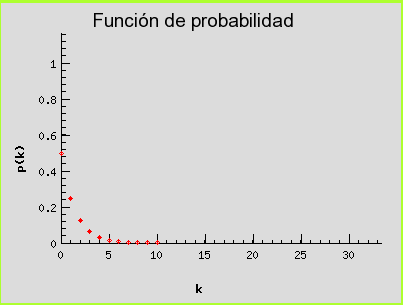
\includegraphics[width=6cm]{images/grafica1.png}
\centering
\caption{Funci�n de probabilidad geom�trica con $p= 0.3$}
\label{imagen}
\end{center}
\end{figure}
\subsection{Funci�n de distribuci�n}
En base de la funci�n de probabilidad se puede expresar la funci�n de distribuci�n de la siguiente manera:
\begin{equation}
F(x)= \sum_{x=1}^{X} q^{x-1} \cdot p
\end{equation}
Desarrollando la expresi�n tendr�amos:
\begin{equation}
F(x)= p \cdot (1+q+q^2+q^3+...+q^{x-1})=p \cdot \frac{1-q^x}{1-q}
\end{equation}
de donde: $F(x)=1-q^x$.
 As� obtenemos la gr�fica de la distribuci�n an�loga a la anterior
\begin{figure}[H]
\begin{center}
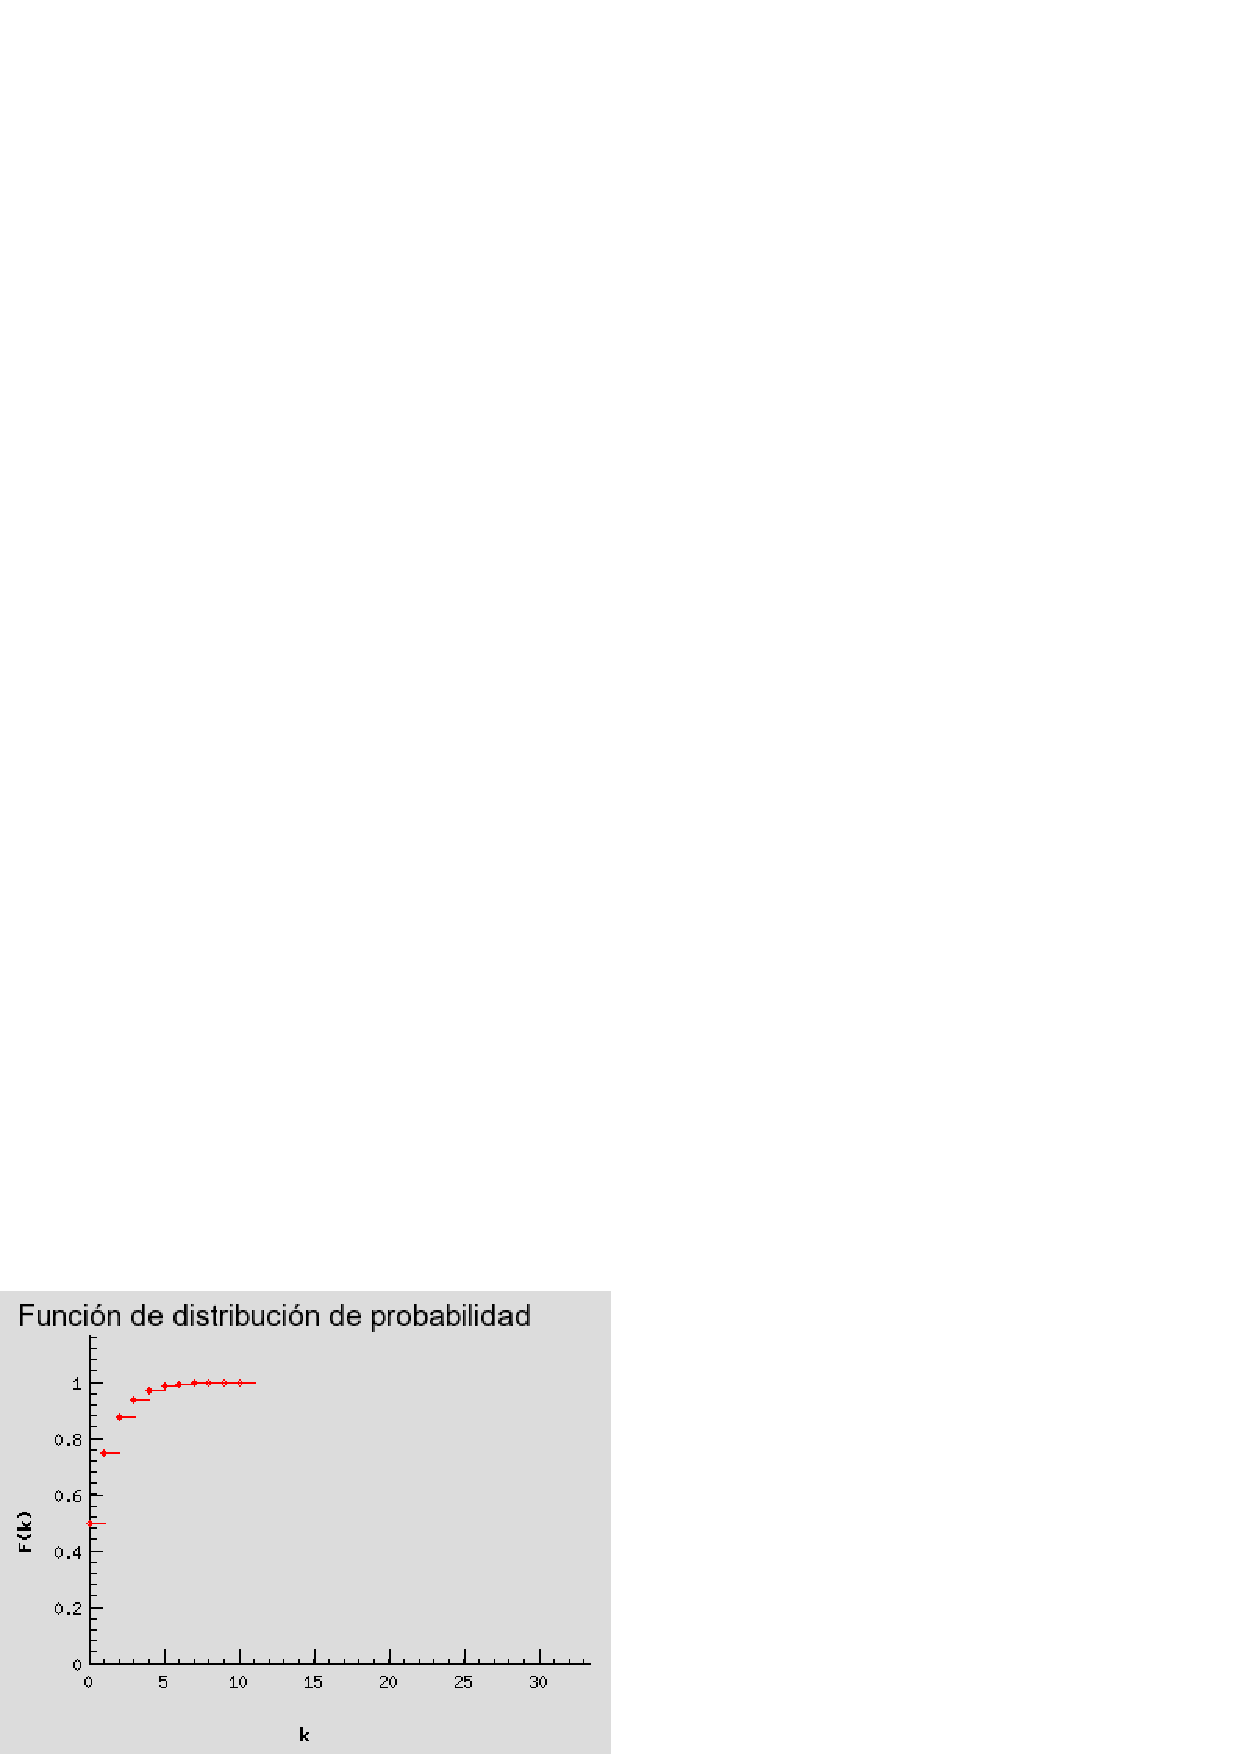
\includegraphics[width=6cm]{images/grafica2.png}
\centering
\caption{Distribuci�n geom�trica con $p= 0.3$}
\label{imagen1}
\end{center}
\end{figure}

\subsection{Propiedades de la geom�trica}
\begin{itemize}
 \item[$\circ$]\bf{La media:} $E(X)=\frac{1}{p}$ o $E(Y)=\frac{1-p}{p}$
 \item[$\circ$]\bf{La varianza:}$var(X)=var(Y)=\frac{1-p}{p^2}$
 \item[$\circ$]\bf{Las funciones generatrices:}
 \begin{center}
 $G_X(s)=\frac{s\cdot p}{1-s(1-p)}$ \hspace{1cm} \text{y} \hspace{1cm} $G_Y(s)=\frac{p}{1-s(1-p)}$, $\; \vert s \vert < (1-p)^{-1}$
 \end{center}
 \item[$\circ$]\textbf{La moda:} es el valor de la variable que tiene asociada mayor probabilidad. Es f�cil comprobar (V�ase la Figura \ref{imagen}) que:
 \[P(x_i)\leq P(x=1) \forall x_i\]
 \item[$\circ$]\bf{La mediana $M_e$:} ser� aquel valor de la variable en el cual la funci�n de distribuci�n toma el valor 0.5. As�: $F(M_e)=1-q^M=\frac{1}{2}\Rightarrow q^M = \frac{1}{2}$
,por lo que, $M_e \cdot ln(q)=ln(1)-ln(2)=-ln(2)\longrightarrow M_e=\frac{-ln(2)}{ln(q)}$
 \item[$\circ$]\bf{Funci�n de Momentos (F.G.M):}
 \begin{equation*}\label{per}
   \begin{split}
     \varphi(t) & =E[e^{tx}]=\sum_{x=1}^{\infty} {e^{tx} \cdot p \cdot q^{x-1}} =\frac{p}{q}\sum_{x=1}^{\infty} {(e^{t} \cdot q)}^x=\lim\limits_{x \rightarrow -\infty}\frac{p}{q}\left( qe^t + (qe^t)^2+...+(qe^t)^x\right)\\
                          & =\lim\limits_{x \rightarrow -\infty}\frac{p}{q} \left[\frac{\cancelto{0}{(qe^t)^{x+1}}-qe^t}{qe^t-1}\right] =\frac{p}{\cancel{q}} \left[\frac{\cancel{q}e^t}{1-qe^t}\right] =p \left[\frac{e^t}{1-qe^t}\right] =\frac{p}{e^{-t}-q}\\
                          & =p(e^{-t}-q)^{-1}
   \end{split}
 \end{equation*}

 Por lo que queda establecida que la F.G.M. tiene la expresi�n:
 \begin{center}
 $\varphi(t)= p(e^{-t}-q)^{-1}$
 \end{center}
\end{itemize}
Siguiendo el ejemplo de las figuras anteriores obtenemos los siguientes resultados:

%------------------------------------------------------------------------------

\begin{table}[H]
\begin{center}
\begin{tabular}{|c|c|c|}
\hline
   \rowcolor[RGB]{0,88,147}    & \textbf{F\'ormula}              & \textbf{Valor para p=0.3} \\ \hline
\textbf{Media} &$E(Y)=\frac{1-p}{p}$ & 1\\ \hline
\textbf{Varianza} & $var(Y)=\frac{1-p}{p^2}$ &2\\ \hline
\textbf{Coeficiente de simetr\'ia} & $G_Y(s)=\frac{p}{1-s(1-p)}$ & 2.1213203435596 \\
\hline
\end{tabular}
\end{center}
\caption{Propiedades geom\'etricas}
\label{tabla}
\end{table}


%------------------------------------------------------------------------------




%%%%%%%%%%%%%%%%%%%%%%%%%%%%%%%%%%%%%%%%%%%%%%%%%%%%%%%%%%%%%%%%%%%%%%%%%%%%%%%
\chapter{Procedimiento experimental}
\label{chapter:exp}

%%%%%%%%%%%%%%%%%%%%%%%%%%%%%%%%%%%%%%%%%%%%%%%%%%%%%%%%%%%%%%%%%%%%%%%%%%%%%%%
% Chapter 3: Procedimiento experimental
%%%%%%%%%%%%%%%%%%%%%%%%%%%%%%%%%%%%%%%%%%%%%%%%%%%%%%%%%%%%%%%%%%%%%%%%%%%%%%%

\leftline{\Large{\bf Introducci�n:}}
En �ste cap�tulo, se describir�n los diversos materiales utilizados en la elaboraci�n y ralizaci�n del algoritmo dise�ados en el software Python. Adem�s, se implementar� el algoritmo de la distribuci�n geom�trica, para observar los procesos en cada paso de ejecuci�n del programa. Finalmente, se expondr�n los resultados finales y las conclusiones que de ellos se desprendan.


%++++++++++++++++++++++++++++++++++++++++++++++++++++++++++++++++++++++++++++++
\section{Descripci�n de los experimentos}
\label{3:sec:1}

%ver el ejmplo del tri�ngulo.

%diagrama de flujo (Buscar el diagrama en latex)
\begin{enumerate}
	 \item \textbf{Distribuci�n Geometrica. }
\begin{description}
  \item[An�lisis:] Vease el cap�tulo 2.
  \item[Formulaci�n] Introducci�n de par�metros: Probabilidad $p$ y n�mero de casos $n$
  \item[Algoritmo: (ver Figura \ref{dflu}).]
\begin{figure}[h!]
  \centering
  % Requires \usepackage{graphicx}
  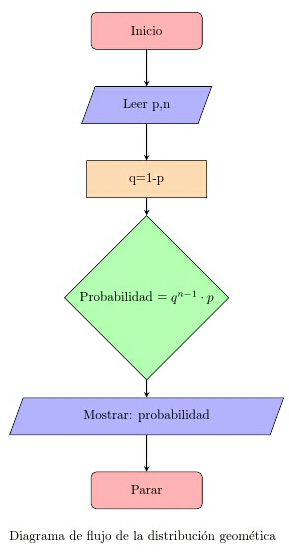
\includegraphics[width=5cm]{images/diafluj.png}
  \caption{Diagrama de Flujo de la Distribuci�n Geom�trica}\label{dflu}
\end{figure}	
  \item[Codifici�n] Vease el c�digo en  en el ap�ndice 1.
\end{description}
\end{enumerate}



%++++++++++++++++++++++++++++++++++++++++++++++++++++++++++++++++++++++++++++++
\section{Descripci�n del material}
\label{3:sec:2}
Tanto para la ejecuci�n en Python, como para la implementaci�n en \LaTeX{}, hemos utilizado:

\begin{enumerate}
	 \item \textbf{Ordenadores:}
%------------------------------------------------------------------------------
\begin{table}[!ht]
\begin{center}
         \scalebox{0.7}{
		\begin{tabular}{|c||c|c|c||}
          \hline
          % after \\: \hline or \cline{col1-col2} \cline{col3-col4} ...
          \rowcolor[RGB]{0,88,147} Marca: &  Modelo: & Procesador: & Sistema Operativo: \\ \hline\hline
          Intel & GenuineIntel & Pentium(R) Dual-Core  CPU      E5300  2.60GHz & Linux-3.2.0-61-generic-i686-with-Ubuntu-12.04-precise\\ \hline
         Acer & Aspire 5735Z & Pentium(R) Dual-Core  CPU      T3200 2.0 GHz & Windows 7 Profesional 32 bits  \\ \hline
          Acer & Aspire 5735 & Pentium(R) Dual-Core  CPU      T3200 2.0 GHz & Windows 7 Profesional 32 bits  \\ \hline
          Asus & Series F55C & Intel (R) Corel (TM) i3-2350M CPU 2.30 GHz & Windows 8.1 64 bits  \\ \hline
        \end{tabular}
        }
\end{center}
        \caption{Modelos de ordenadores y procesadores:}
        \label{marca:2}
\end{table}




%------------------------------------------------------------------------------


  \item \textbf{Versi�n de Python:}
  Para la realizaci�n del programa que soluciona los distintos problemas, anteriormente descritos, utilizaremos la siguiente versi�n de Python:
  \begin{center}
  \textbf{PYTHON 2.7.3 [GCC 4.6.3] ON LINUX2}
  \end{center}

  \item \textbf{Versiones de \LaTeX{}}
  As� mismo hemos utilizado las siguientes versiones de \LaTeX{} y distintos entornos de trabajo:\footnote{Ambos entornos, trabajan en el sistema operativo Windos (en sus distintas versiones, dadas en el cuadro \ref{marca:2})}
%------------------------------------------------------------------------------
\begin{table}[!ht]
\begin{center}

		\begin{tabular}{|c||c||}
          \hline
          % after \\: \hline or \cline{col1-col2} \cline{col3-col4} ...
          \rowcolor[RGB]{0,88,147} Version Miktex: &  Editor texto: \\ \hline\hline
           2.9 & TexMaker   \\ \hline
         2.9 & WinEdt 8.0    \\ \hline
        \end{tabular}

\end{center}
        \caption{Versiones de \LaTeX{}}
        \label{marca:1}
\end{table} 
%------------------------------------------------------------------------------



\end{enumerate}


%++++++++++++++++++++++++++++++++++++++++++++++++++++++++++++++++++++++++++++++
\newpage
\section{Resultados obtenidos:}
\label{3:sec:3}

Para la realizaci�n de la siguiente tabla \ref{tab:1}, nos hemos ayudado de los problemas resueltos en el cap�tulo 1. Se ha a�adido el c�lculo del error entre los resultados obtenidos, por el programa dise�ado en Python, en comparaci�n con los resultados obtenidos : ''a mano'' y con una calculadora online \cite{URL:XML}

%------------------------------------------------------------------------------
%--------------------------------------------------------------------------
\begin{table}[!ht]
\begin{center}
\begin{tabular}{|c|c|} \hline 
\textbf{Tiempo  } & \textbf{Velocidad} \\ 
\textbf{($\pm$ 0.001 s)} & \textbf{($\pm$ 0.1 m/s)} \\ \hline \hline
1.234 &
67.8
\\
\hline

2.345 &
78.9
\\
\hline

3.456 &
89.1
\\
\hline

4.567 &
91.2
\\
\hline

\end{tabular}
\end{center}
\caption{Resultados experimentales de tiempo (s) y velocidad (m/s)}
\label{tab:1}
\end{table}


%------------------------------------------------------------------------------

%parrafo del tiempo

Vamos a comprobar la eficacia (en tiempo de ejecuci�n) de nuestro programa Python, para cada unos de sus casos individualmente, es decir, para los casos:
\begin{enumerate}
 \item Caso $P(X=n)$
 \item Caso $P(X\leq n)$
 \item Caso $P(X<n)$
 \item Caso $P(X\geq n)$
\end{enumerate}
Los resultados se recogen en la siguiente tabla:
%------------------------------------------------------------------------------
\begin{table}[!ht]
\begin{center}
\scalebox{0.6}{
\begin{tabular}{|c|l|l|c|}
\hline
\rowcolor[RGB]{0,88,147} \textbf{Problemas:  } & \textbf{p:} &\textbf{Tipo de problemas:} & \textbf{Tiempo de ejecuci\'on: } \\ \hline
 1 & 0.5 & $P(X\geq 2)$ & 0.000047 \\
 2 & 0.8 & $P(X=1)$ & 0.000007 \\
   & 0.8 & $P(X=2)$ & 0.000035\\
   & 0.8 & $P(X=3)$ & 0.000035\\
   & 0.8 & $P(X=4)$ & 0.000035\\
   & 0.8 & $P(X=5)$ & 0.000048\\
   & 0.8 & $P(X\leq 5)$ & 0.000045 \\
 3 & 0.16666666 & $P(X=3)$ & 0.000035\\
 4 & 0.4 & $P(X<3)$ & 0.000044\\
 \hline
\end{tabular}
}
\end{center}
\caption{Tabla del c\'alculo del tiempo.}
\end{table} 
%------------------------------------------------------------------------------
% parrafo de la grafica
A continuaci�n se muestra los datos obtenidos (tiempo de compilaci�n), los cuales var�an atendiendo a los diferentes valoras de n. \footnote{Para simplificar el trabajo todas las funciones tendr�n los mismos valores de p ($p=0.3$)}

%------------------------------------------------------------------------------
\begin{figure}[!th]
\begin{center}
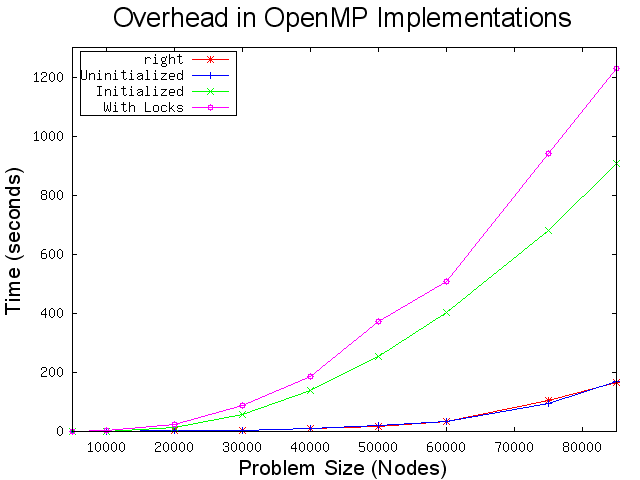
\includegraphics[width=0.7\textwidth]{images/figura1.png}
\caption{Ejemplo de figura}
\label{fig:1}
\end{center}
\end{figure}
%------------------------------------------------------------------------------




%++++++++++++++++++++++++++++++++++++++++++++++++++++++++++++++++++++++++++++++
\section{An�lisis de los resultados}
\label{3:sec:4}

Como se puede observar en la tabla \ref{tabla:1} los errores que se producen entre la funci�n implementada en Python y la calculadora de precisi�n, o las operaciones ''echas a mano'', es m�nima. Esta observaci�n nos induce a afirmar que esta funci�n tiene un grado de exactitud muy alto, y por consiguiente podr�amos utilizarla en cualquier problema con el mismo esquema que los estudiados en este estudio.

Adem�s,  (se analizar� despu�s de haber creado toda la gr�fica y se estudiar� en su conjunto).

%%%%%%%%%%%%%%%%%%%%%%%%%%%%%%%%%%%%%%%%%%%%%%%%%%%%%%%%%%%%%%%%%%%%%%%%%%%%%%%
\chapter{Conclusiones}
\label{chapter:conclusiones}

%%%%%%%%%%%%%%%%%%%%%%%%%%%%%%%%%%%%%%%%%%%%%%%%%%%%%%%%%%%%%%%%%%%%%%%%%%%%%
% Chapter 4: Conclusiones y Trabajos Futuros
%%%%%%%%%%%%%%%%%%%%%%%%%%%%%%%%%%%%%%%%%%%%%%%%%%%%%%%%%%%%%%%%%%%%%%%%%%%%%%%
Tras el estudio y ejecuci\'on de varios tipos de problemas sobre la Distribuci\'on Geom\'etrica, se puede observar que:\\
\begin{enumerate}
	 \item Se nos asign\'o en este trabajo  hacer un programa Python que solucionara la funci\'on de probabilidad de la distribuci\'on geom\'etrica, para ello, tuvimos que buscar informaci\'on sobre esta distribuci\'on (def calcular geo1).

\item Despu\'es iniciamos la implementaci\'on de la funci\'on de la probabilidad, para ello creamos una funci\'on (def calcular\_geo).
   Esta funci\'on nos era \'util en alguno de los problemas, pero no en otros casos. \'Este problema lo solucionamos mediante ensayo y error, resolviendo as\'i nuestro dilema incorporando una nueva funci\'on.
  \item Podemos sacar como conclusi\'on final que:
   \begin{enumerate}
   	 \item Debemos ejecutar varias veces un programa, hasta purificarlo y sacar un programa eficiente y operativo.

     \item Adem\'as, gracias a nuestra b\'usqueda de informaci\'on hemos podido refrescar y ampliar conocimientos sobre probabilidades, m\'as concretamente sobre la distribuci\'on geom\'etrica.
     \item Nos hemos dado cuenta del enorme potencial que tiene la utilizaci\'on de \LaTeX, Beamer y Python, para la elaboraci\'on documental, de presentaci\'on y de creaci\'on de algoritmos, respect\'ivamente. Nos ser\'a de gran ayuda en la elaboraci\'on de nuestros escritos, en el marco de nuestra formaci\'on acad\'emica universitaria y laboral.
   \end{enumerate}

\end{enumerate}






%%%%%%%%%%%%%%%%%%%%%%%%%%%%%%%%%%%%%%%%%%%%%%%%%%%%%%%%%%%%%%%%%%%%%%%%%%%%%%%

%%%%%%%%%%%%%%%%%%%%%%%%%%%%%%%%%%%%%%%%%%%%%%%%%%%%%%%%%%%%%%%%%%%%%%%%%%%%%%%
\newpage{\pagestyle{empty}\cleardoublepage}
\thispagestyle{empty}
\begin{appendix}

\chapter{T�tulo del Ap�ndice 1}
\label{appendix:1}

\section{Algoritmo Principal:}
\label{Apendice1:XXX}

\begin{center}
\begin{footnotesize}
\begin{verbatim}
###################################################################################
# sol_geo.py
###################################################################################
#
# AUTORES: Maria Baeza Lopez
#          Juan Jesus Doniz Labrador
#          Jesus Manuel Rodriguez Falcon
#
# FECHA: 09/05/2014
#
# DESCRIPCION: Este programa realiza el calculo de la Distribucion Geometrica, dados los
#			   parametros de entrada n y p, utilizando el modulo: mod_geo.py.
#              Este programa da 4 opciones al usuario para el calculo de dicha distribucion:
#			   (0=P(X=n),1=P(X<=n,2=P(X<n),3=P(x>=n))
#
###################################################################################

#!/usr/bin/python
#!encoding: UTF-8
import sys
import mod_geo
import time
import timeit
# Menu principal
argumentos = sys.argv[1:]
 # print argumentos         Imprime la lista con los parametros que le des desde la consola
if (len(argumentos) == 2):# si la lista es de dos elementos (n,p)
  n = int(argumentos[0])
  p = float(argumentos[1])
else:
    print "Introduzca el n de pruebas necesarias para obtener un exito (n>0):"
    n = int (raw_input())
    print "Introduzca el valor p (p>0):"
    p = float(raw_input())
if (n > 0):
  print "¿Que tipo de probabilidad vas a hallar? (0=P(X=n), 1=P(X<=n), 2=P(X<n), 3=P(X>=n))"
  respuesta=int(raw_input())
  if (respuesta==0):
    start=time.time()
    probabilidad=mod_geo.calcular_geo (n,p)
    finish=time.time()-start
    print "La probabilidad P[X= %d] con p= %f es: %f y 
           he tardado %f segundos en calcularlo"  %(n,p,probabilidad,finish)
  elif (respuesta==1):
    start=time.time()
    probabilidad=mod_geo.calcular_geo1(n,p)
    finish=time.time()-start

    print "La probabilidad P[X<= %d] con p= %f es: %f y 
           he tardado %f segundos en calcularlo"  %(n,p,probabilidad,finish)
  elif (respuesta == 2):
    start=time.time()                        
    probabilidad=mod_geo.calcular_geo1(n-1,p)
    finish=time.time()-start                 

    print "La probabilidad P[X< %d] con p= %f es: %f y 
           he tardado %f segundos en calcularlo"  %(n,p,probabilidad,finish)
  else:
    start=time.time()                       
    prob=mod_geo.calcular_geo1(n,p)
    probabilidad = 1 - prob
    finish=time.time()-start                 

    print "La probabilidad P[X>= %d] con p= %f es: %f y 
           he tardado %f segundos en calcularlo"  %(n,p,probabilidad,finish)

else:
    print "No podemos hallar la probabilidad"


\end{verbatim}
\end{footnotesize}
\end{center}

\newpage
\section{Algoritmo del Modulo:}
\label{Apendice1:YYY}

\begin{center}
\begin{footnotesize}
\begin{verbatim}
###################################################################################
# mod_geo.py
###################################################################################
#
# AUTORES: Maria Baeza Lopez
#          Juan Jesus Doniz Labrador
#          Jesus Manuel Rodriguez Falcon
#
# FECHA: 09/05/2014
#
# DESCRIPCION: Este modulo contiene dos funciones:
#             1. calcular_geo (n,p)---->calcula la probabilidad geometrica
#			  y la devuelve a sol_geo.py
#             2. calcular_geo1 (n,p)--->Calcula la probabilidad geometrica
#             desde 1 hasta n y las va almacenando en sumaprobabilidad
#
###################################################################################

#!/usr/bin/python
#!encoding: UTF-8
import sys
import math

def calcular_geo (n,p):
  if (n>1):
    q=1-p
    probabilidad=(q**(n-1))*p
  else:
    probabilidad=p
  return (probabilidad)

def calcular_geo1 (n,p):
  probabilidad=0
  for i in range (1,n+1):
    sumaprobabilidad=calcular_geo(i,p)
    probabilidad+=sumaprobabilidad
  return (probabilidad)
\end{verbatim}
\end{footnotesize}
\end{center}


\chapter{T�tulo del Ap�ndice 2}
\label{appendix:2}

\section{C\'odigo para generar gr\'aficas}
\label{Apendice2:label}

\begin{center}
\begin{footnotesize}

\begin{verbatim}
#!/usr/bin/python
#! enconding: UTF-8

import pylab as dibujo

x = [20,40,60,80,100]
y1 = [0.000051,0.000045,0.000046,0.000046,0.000048]
y2 = [0.000095,0.000112,0.000133,0.000158,0.000183]
y3 = [0.000086,0.000112,0.000134,0.000159,0.000185]
y4 = [0.000089,0.000113,0.000139,0.000164,0.000188]

dibujo.title ('Tiempo')

dibujo.plot (x, y1,linestyle='-.',marker='*',color='r', label='Para el caso 0')  #':' '--' '_' . 
Los colores son 'r'  junto a m b g c y.    Los marker son 'o' junto a s p * + . ^
dibujo.plot (x, y2,linestyle='--',marker='*',color='b', label='Para el caso 1')
dibujo.plot (x, y3,linestyle='-',marker='*',color='g', label='Para el caso 2')
dibujo.plot (x, y4,linestyle=':',marker='*',color='m', label='Para el caso 3')

dibujo.legend()      # Esto se pone para que aparezca la leyenda de las lineas
dibujo.xlim(10,155)
dibujo.ylim(0.000044,0.000190)
dibujo.xticks(x)
dibujo.xlabel ('Valores de la n')
dibujo.ylabel ('Tiempo en segundos')

dibujo.show()
\end{verbatim}

\end{footnotesize}
\end{center}


\end{appendix}

%%%%%%%%%%%%%%%%%%%%%%%%%%%%%%%%%%%%%%%%%%%%%%%%%%%%%%%%%%%%%%%%%%%%%%%%%%%%%%%
\addcontentsline{toc}{chapter}{Bibliograf�a}
\bibliographystyle{plain}


\bibliography{bib/references}
\nocite{*}

%%%%%%%%%%%%%%%%%%%%%%%%%%%%%%%%%%%%%%%%%%%%%%%%%%%%%%%%%%%%%%%%%%%%%%%%%%%%%%%

\end{document}
